
\documentclass[11pt,twocolumn]{article}

\usepackage[paperheight=297mm,paperwidth=210mm,top=5mm,bottom=25mm,left=25mm,right=25mm]{geometry}

\usepackage{txfonts}
\usepackage{graphicx}
\usepackage[T1]{fontenc}
\usepackage[icelandic]{babel}
\usepackage{listings}
\usepackage[utf8]{inputenc}
\usepackage[bf]{caption}
\graphicspath{{./}}


\setlength{\baselineskip}{0pt} 
\setlength{\parindent}{0pt}
\setlength{\parskip}{0pt}

\usepackage{graphicx}
\title{ Heimadæmi 6 - Tölvugrafík }
\date{}

\author{Davíð Isebarn Ágústsson }
\begin{document}
\maketitle

Dæmin eru öll inná:

https://notendur.hi.is/~dia2/203M/HD/HD6/

\paragraph{Dæmi 1}
sjá viewpoints.html

\paragraph{Dæmi 2}
sjá PhongTepottur.html

\paragraph{Dæmi 3}
sjá PhongTepottur2.html

\paragraph{Dæmi 4}
----------------------------->

\paragraph{Dæmi 5}
sjá flag.html


\newpage

\paragraph{Dæmi 4}

\

Til að hámarka gildi dreifiendurskins þá þarf þverstefnuvigurinn að snúa beint að stefnu ljósgjafans svo að ljósið lendi "akkúrat" flatt. Sá liður er ekki háður staðsetningu athugandans.

Depilendurskinið er öðruvísi en þar er skynjaður styrkur háður staðsetningu athuganda

Þegar ljósvigur lendir á fleti undir horni A, þá speglast ljósvigurinn þannig að ef á milli
normalvigurs á flötinn og ljósvigurs er horn B (A+B = 90) þá fer endurspeglunarvigurinn
eftir sama horni í burtu (eða réttara sagt undir horni A+90) 
Athugandi sem er staddur inni í þessum vigri sér hámarksendurskyn, sem dofnar sem horninu er breytt lengra frá speglunarvigrinum

Nú er ljósvigurinn skilgreindur sem l og stefna áhorfanda sem v
Við viljum að stefna áhorfanda sé sú sama og endurskynsvigursins, en þá verðum við að finna réttann normalvigur, til þess að afstaða punktsins sé rétt

Við viljum því að stefna normalvigursins sé akkúrat mitt á milli ljósvigursins og stefnu áhorfandans, en hornið milli tveggja vigra er skilgreint sem

\[
C = \cos^{-1}\frac{i\cdot v}{||i||||v||}
\]

og við viljum fá hornið akkúrat á milli svo við fáum C/2 m.v normalvigur

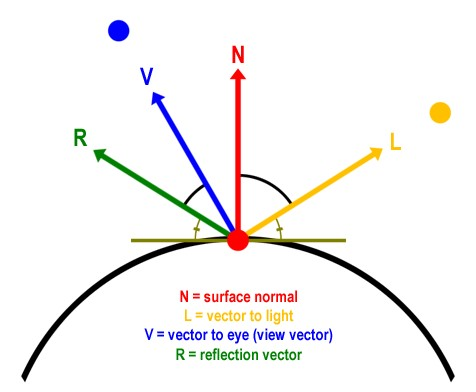
\includegraphics[width = \linewidth]{1.jpg}

Á myndinni er athugandi aðeins fyrir ofan endurskynsvigurinn, en ef hann færði sig niður í hann þá sæi hann hámarksendurskin í rauða punktinum

\end{document}